\chapter{MATERIAIS E MÉTODOS} % ou PROCEDIMENTOS METODOLÓGICOS
\label{chap:metodologia}

Procedimentos Metodológicos relaciona-se aos passos percorridos para responder as questões de pesquisa. Deve ser detalhado o suficiente para que outro pesquisador possa reproduzir o caminho percorrido, buscando atender às características de replicabilidade e verificabilidade da ciência. Mesmo quando não é cabível se reproduzir o estudo com as mesmas pessoas, a possibilidade de replicação do método com um público diferente é característica fundamental para a evolução do conhecimento na área. 

Descrevem-se detalhadamente as etapas para a realização da pesquisa, incluindo o campo da pesquisa e a amostra de dados considerada.  Da mesma forma que uma receita culinária, ou a descrição de um algoritmo, o método científico tem uma linguagem própria a ser seguida e é preciso cumprir as tradições de cada área de pesquisa para que os resultados sejam considerados válidos.

Cada etapa da realização do trabalho deverá responder informar aspectos como: 1) objetivo da etapa, materiais utilizados, métodos de trabalho, e campo de estudo. O campo é o local onde serão coletados os dados, devendo-se informar onde, quem, e quando ocorrerá. Quando aplicável, faça referências a apêndices do seu trabalho contendo os instrumentos de coleta de dados a serem utilizados.

Cada comunidade científica possui diferentes métodos para investigar a realidade. As técnicas de pesquisa mudam conforme a natureza do estudo e de sua área, sejam elas relacionadas à coleta ou ao registro de dados.

Seguem alguns exemplos:

\begin{alineascomponto}
    	\item Experimentos, o que inclui desenvolvimento de protótipos ou produtos;
        \item Análise de documentos;
        \item Entrevistas, em duas diversas variações;
        \item Observações, em suas diversas variações.    
\end{alineascomponto}

Estas são apenas orientações gerais. É fundamental consultar o orientador quando às prática comuns para a área temática do trabalho

\section{Título da seção secundária}

Em caso de trabalhos com coleta de dados em campo, típico de áreas como IHC e gestão, por exemplo, esta seção contém a metodologia da pesquisa. Em caso de trabalhos mais voltados para desenvolvimento, ou mais ligados à matemática, esta seção será mais breve, se houver, contendo a descrição geral dos passos realizados. 

As ilustrações (fotografias, gráficos, mapas, plantas, quadros) e tabelas devem ser citados e inseridos o mais próximo possível do trecho a que se referem. O título de ilustrações  deve estar alinhado à sua esquerda; se a ilustração for pequena, pode-se adicionar uma moldura para o resultado ficar esteticamente melhor.

Figuras devem ser legíveis, ao contrário da forma como está exibida a Figura \ref{figura-1}.  

\begin{figure}[htbp]
	\centering
	\IBGEtab{
		\Caption{\label{figura-1}Organização do conhecimento/Representação do conhecimento, Organização da informação/Representação da informação}		
    }{
		\fbox{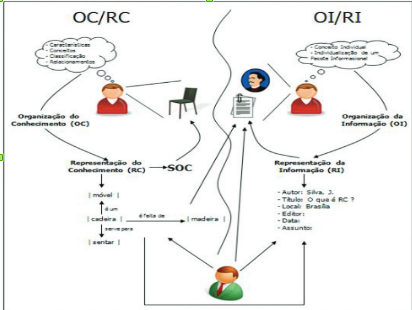
\includegraphics[scale=1.0]{figuras/figura-1}}
	}{
	\Fonte{\citeonline{smit2010temas}}
}
\end{figure}

\lipsum[1]

\begin{figure}[htbp]
	\centering
	\IBGEtab{
		\Caption{\label{figura-1}Ciclo da informação}		
    }{
		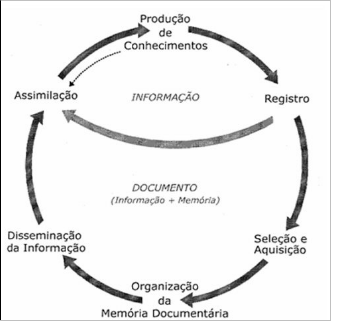
\includegraphics[scale=0.8]{figuras/figura-2}
	}{
	\Fonte{\citeonline{tristao2004sistema}}
}
\end{figure}


